\paragraph{Sơ đồ tuần tự luồng xác nhận liên kết từ email}

Luồng nghiệp vụ này mô tả
quá trình xác thực token
khi người dùng click
vào liên kết khôi phục trong email,
nhận phiên đăng nhập từ callback
và tiếp tục qua bước MFA trước khi
được chuyển tới trang đổi mật khẩu của ứng dụng.

\begin{figure}[H]
\centering
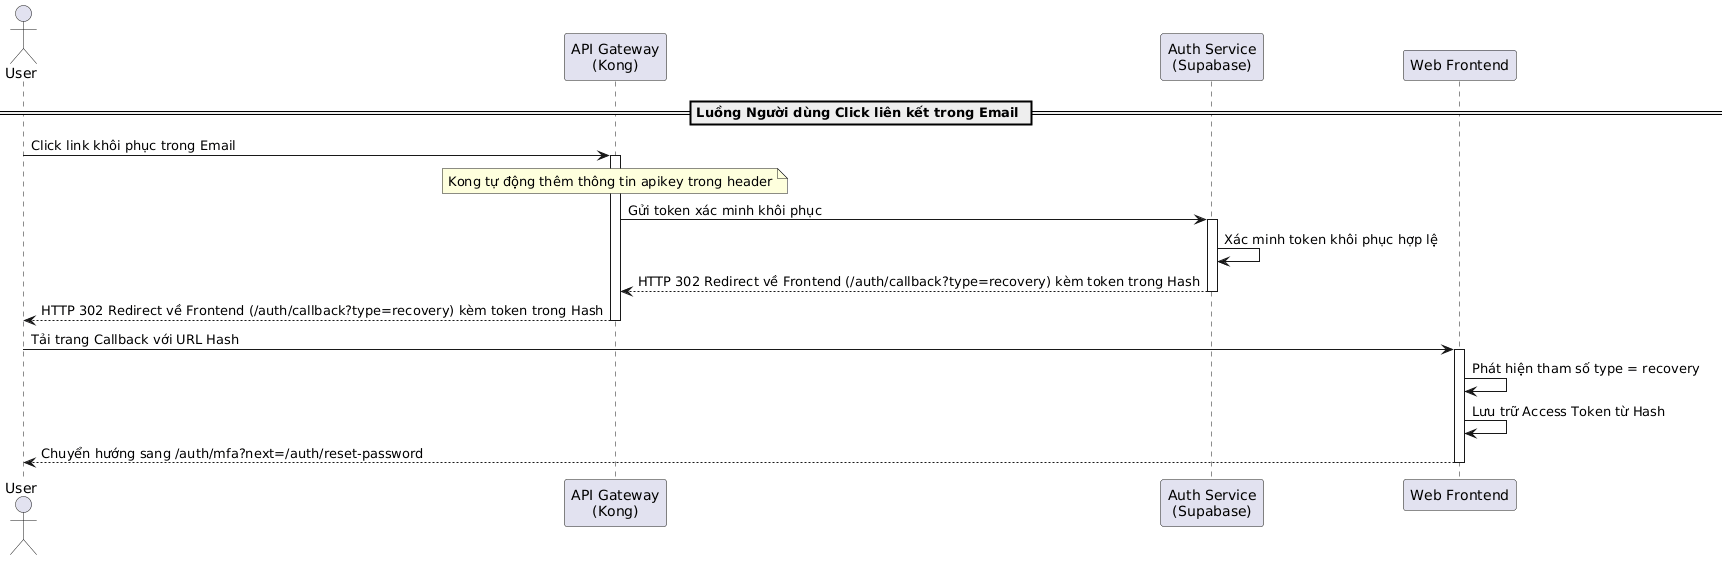
\includegraphics[width=0.95\textwidth]{contents/Sequence/UML-Sequence-UserEmailLinkVerificationRedirect.png}
\caption{Sơ đồ tuần tự luồng xác nhận liên kết từ email}
\end{figure}

\begin{table}[H]
\centering
\renewcommand{\arraystretch}{1.3}

\begin{tabular}{|l|l|p{5cm}|}
\hline
\textbf{Thành phần} & \textbf{Phân loại} & \textbf{Vai trò trong hệ thống} \\ \hline
User & Actor & Người dùng click liên kết xác nhận. \\ \hline
API Gateway (Kong) & Component & Cổng API chuyển tiếp các yêu cầu API. \\ \hline
Auth Service (Supabase) & Microservice & Dịch vụ Supabase xác minh token khôi phục và trả về HTTP 302 Redirect. \\ \hline
Web Frontend & Component & Giao diện web Next.js. \\ \hline
\end{tabular}
\caption{Các thành phần tham gia luồng xác nhận liên kết từ email}
\end{table}

\subparagraph{Mô tả tổng quan}

\begin{itemize}

\item \textbf{Nhấp liên kết xác nhận:}
Người dùng nhấn vào
liên kết xác thực trong thư điện tử.
Yêu cầu được gửi qua cổng API
tới Auth Service để kiểm tra tính hợp lệ của mã xác nhận.

\item \textbf{Chuyển hướng trình duyệt:}
Nếu mã hợp lệ, Auth Service trả về yêu cầu
chuyển hướng trình duyệt của người dùng đến trang tiếp nhận của giao diện
kèm theo mã xác thực tạm thời trong địa chỉ trang web.

\item \textbf{Xác thực hai lớp:}
Giao diện nhận phản hồi,
lưu trữ mã xác thực tạm thời và chuyển hướng người dùng sang trang đổi mật khẩu.
Sau khi vượt qua bước xác thực hai lớp, hệ thống mới cho phép người dùng đặt lại mật khẩu mới.
\end{itemize}
